\section{Resultados e discussão}\label{sec:resultados}

\subsection{Plataforma computacional}\label{sec:plataforma}

Como principal produto de engenharia deste trabalho, foi desenvolvida uma plataforma computacional de acesso livre para o dimensionamento de pontes de madeira, capaz de realizar a verificação completa dos elementos estruturais em conformidade com as ABNT NBR 7190 \parencite{NBR7190-1:2022} e NBR 7188 \parencite{nbr7188}, disponível nos idiomas português e inglês \parencite{ReliaBridge2026}. A interface, ilustrada nas Figuras~\ref{fig:tela_inicial} e~\ref{fig:interface_dim}, é organizada em módulos que permitem a navegação sequencial entre as etapas de dimensionamento por otimização, projeto detalhado dos elementos e análise dos resultados. Ao final do processamento, a ferramenta disponibiliza para download a planilha de dados de entrada, os resultados do pré-dimensionamento e a imagem da fronteira de Pareto.

\begin{figure}[!ht]
    \centering
    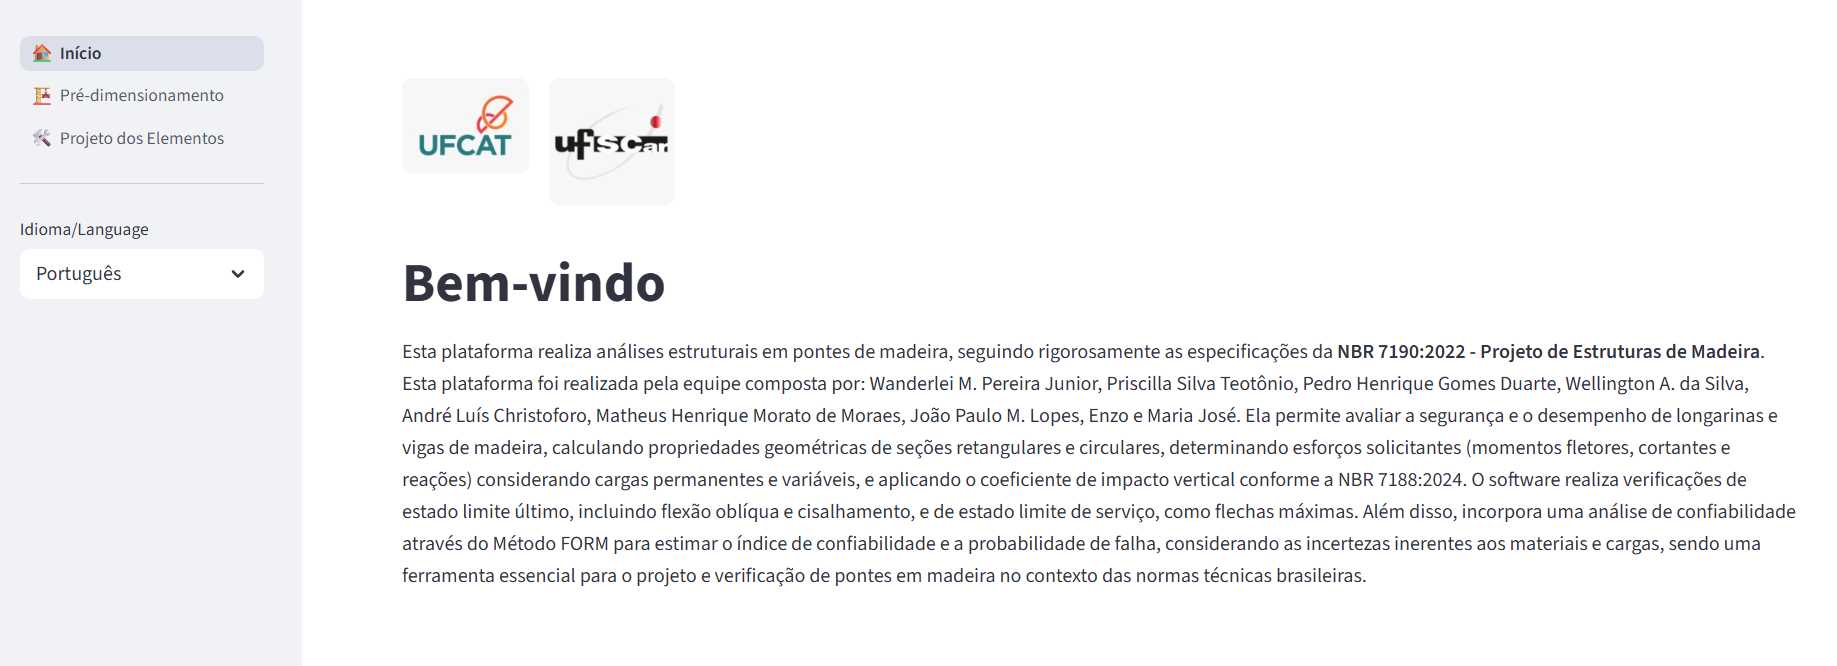
\includegraphics[width=0.85\textwidth]{figuras/interface_inicial.png}
    \caption{Tela inicial da plataforma computacional.}
    \label{fig:tela_inicial}
\end{figure}

\begin{figure}[!ht]
    \centering
    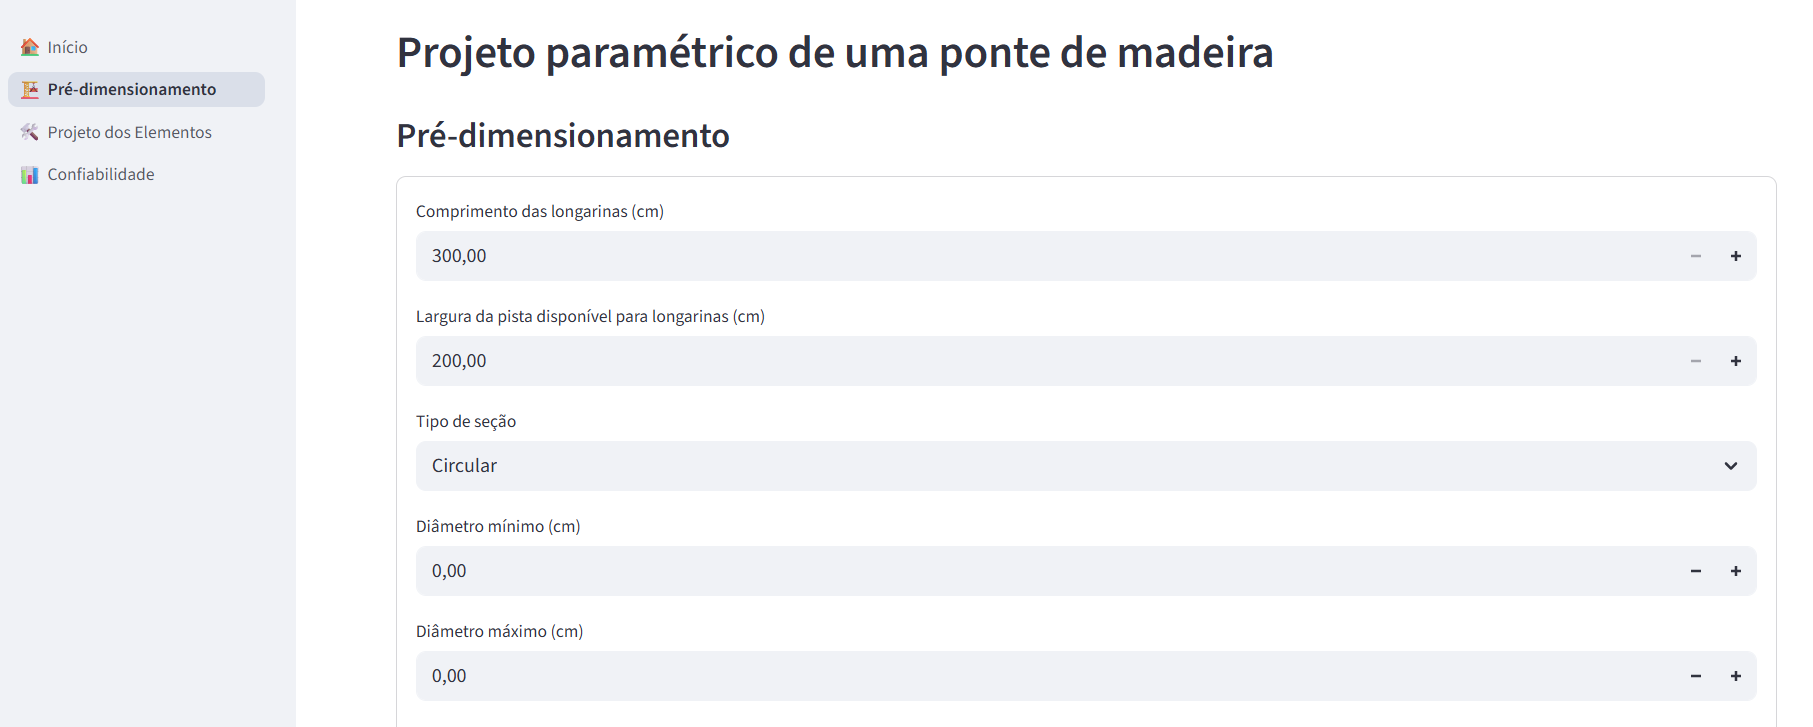
\includegraphics[width=0.9\textwidth]{figuras/interface_dimensionamento.png}
    \caption{Módulo de dimensionamento por otimização.}
    \label{fig:interface_dim}
\end{figure}

\subsection{Definição dos casos de estudo}\label{sec:casos}

Para avaliar o desempenho da metodologia, foram consideradas duas pontes hipotéticas de estrada vicinal com a mesma configuração geométrica e as mesmas propriedades mecânicas, diferenciando-se exclusivamente pelo trem tipo adotado. Os parâmetros fixos são apresentados na Tabela~\ref{tab:parametros}, e os carregamentos móveis de cada cenário na Tabela~\ref{tab:carregamento}. A Ponte 01 foi dimensionada para o trem tipo TB-240 e a Ponte 02 para o TB-450. Os intervalos das variáveis de projeto adotados na otimização são apresentados na Tabela~\ref{tab:intervalos}.

\begin{table}[!ht]
\caption{Parâmetros geométricos, mecânicos e coeficientes adotados nas análises.\label{tab:parametros}}
\begin{threeparttable}
\begin{tabular*}{\columnwidth}{@{\extracolsep\fill}lc@{\extracolsep\fill}}
\toprule
Parâmetro & Valor \\
\midrule
Comprimento das longarinas, $L$ (cm) & 500 \\
Largura da pista, $b_{w,\mathrm{pista}}$ (cm) & 900 \\
Carga permanente distribuída, $p_{gk}$ (kPa) & 1 \\
Distância entre eixos, $a$ (m) & 1{,}5 \\
Classe de carregamento & Permanente \\
Classe da madeira & Madeira natural \\
Classe de umidade & 1 \\
Coeficiente parcial das ações permanentes, $\gamma_g$ & 1{,}35 \\
Coeficiente parcial das ações variáveis, $\gamma_q$ & 1{,}50 \\
Coeficiente de minoração (tensões normais), $\gamma_{wf}$ & 1{,}40 \\
Coeficiente de minoração (cisalhamento), $\gamma_{wc}$ & 1{,}80 \\
Fator de combinação quase permanente, $\psi_2$ & 0{,}30 \\
Coeficiente de fluência, $\varphi$ & 0{,}60 \\
Densidade da madeira (kg/m\textsuperscript{3}) & 620 \\
Resistência característica à flexão, $f_{mk}$ (MPa) & 50 \\
Resistência característica ao cisalhamento, $f_{vk}$ (MPa) & 4 \\
Módulo de elasticidade à flexão, $E_{0,\mathrm{ef}}$ (GPa) & 14 \\
\bottomrule
\end{tabular*}
\end{threeparttable}
\end{table}

\begin{table}[!ht]
\caption{Cargas móveis para cada trem tipo.\label{tab:carregamento}}
\begin{threeparttable}
\begin{tabular*}{\columnwidth}{@{\extracolsep\fill}lcc@{\extracolsep\fill}}
\toprule
Parâmetro & TB-240 (Ponte 01) & TB-450 (Ponte 02) \\
\midrule
Carga concentrada por roda, $p_{rodak}$ (kN) & 40 & 75 \\
Carga variável distribuída, $p_{qk}$ (kPa) & 4 & 5 \\
\bottomrule
\end{tabular*}
\end{threeparttable}
\end{table}

\begin{table}[!ht]
\caption{Intervalos adotados para as variáveis de projeto.\label{tab:intervalos}}
\begin{threeparttable}
\begin{tabular*}{\columnwidth}{@{\extracolsep\fill}lcc@{\extracolsep\fill}}
\toprule
Variável & Valor mínimo (cm) & Valor máximo (cm) \\
\midrule
Diâmetro da longarina, $d$ & 30 & 150 \\
Espaçamento entre longarinas, $esp$ & 30 & 200 \\
Largura da prancha do tabuleiro, $b_w$ & 5 & 60 \\
Altura da prancha do tabuleiro, $h$ & 5 & 60 \\
\bottomrule
\end{tabular*}
\end{threeparttable}
\end{table}

\subsection{Fronteira eficiente da Ponte 01 (TB-240)}\label{sec:ponte01}

A otimização robusta multiobjetivo da Ponte 01 gerou um conjunto de soluções viáveis distribuídas ao longo da fronteira eficiente. A Tabela~\ref{tab:solucoes01} apresenta uma amostra representativa das soluções obtidas, com as respectivas funções objetivo e valores das funções limite das restrições, todas negativas, o que confirma o atendimento aos critérios normativos mesmo sob a avaliação robusta.

\begin{table}[!ht]
\caption{Soluções representativas da fronteira eficiente da Ponte 01 (TB-240).\label{tab:solucoes01}}
\begin{threeparttable}
\setlength{\tabcolsep}{3pt}
\begin{tabular*}{\textwidth}{@{\extracolsep{\fill}}ccccccc@{\extracolsep{\fill}}}
\toprule
$d$ (cm) & $esp$ (cm) & $h$ (cm) & Área (m\textsuperscript{2}) & $\delta_{\mathrm{tot}}/(L/250)$ & Flex. long. & Flecha long. \\
\midrule
43{,}74 & 30{,}79 & 5{,}00 & 0{,}153 & 0{,}234 & $-0{,}000$ & $-0{,}363$ \\
44{,}16 & 76{,}36 & 18{,}27 & 0{,}162 & 0{,}244 & $-0{,}000$ & $-0{,}387$ \\
44{,}72 & 118{,}71 & 28{,}03 & 0{,}171 & 0{,}256 & $-0{,}001$ & $-0{,}417$ \\
45{,}26 & 154{,}59 & 35{,}09 & 0{,}178 & 0{,}267 & $-0{,}000$ & $-0{,}444$ \\
45{,}74 & 186{,}92 & 38{,}89 & 0{,}184 & 0{,}276 & $-0{,}000$ & $-0{,}467$ \\
46{,}27 & 200{,}00 & 49{,}07 & 0{,}193 & 0{,}286 & $-0{,}000$ & $-0{,}491$ \\
46{,}63 & 196{,}40 & 59{,}91 & 0{,}201 & 0{,}292 & $-0{,}000$ & $-0{,}507$ \\
\bottomrule
\end{tabular*}
\end{threeparttable}
\end{table}

A fronteira eficiente é apresentada na Figura~\ref{fig:fronteira01}, que relaciona a área total de madeira com a flecha total adimensional. Observa-se uma tendência crescente entre as variáveis, evidenciando o compromisso típico entre rigidez e economia de material. Para valores de flecha adimensional da ordem de 0{,}24, correspondentes a soluções mais rígidas, a área total é de aproximadamente 0{,}16~m\textsuperscript{2}; já para soluções próximas ao limite admissível de serviço (flecha adimensional próxima de 0{,}29), a área total demandada é da ordem de 0{,}20~m\textsuperscript{2}.

\begin{figure}[!ht]
    \centering
    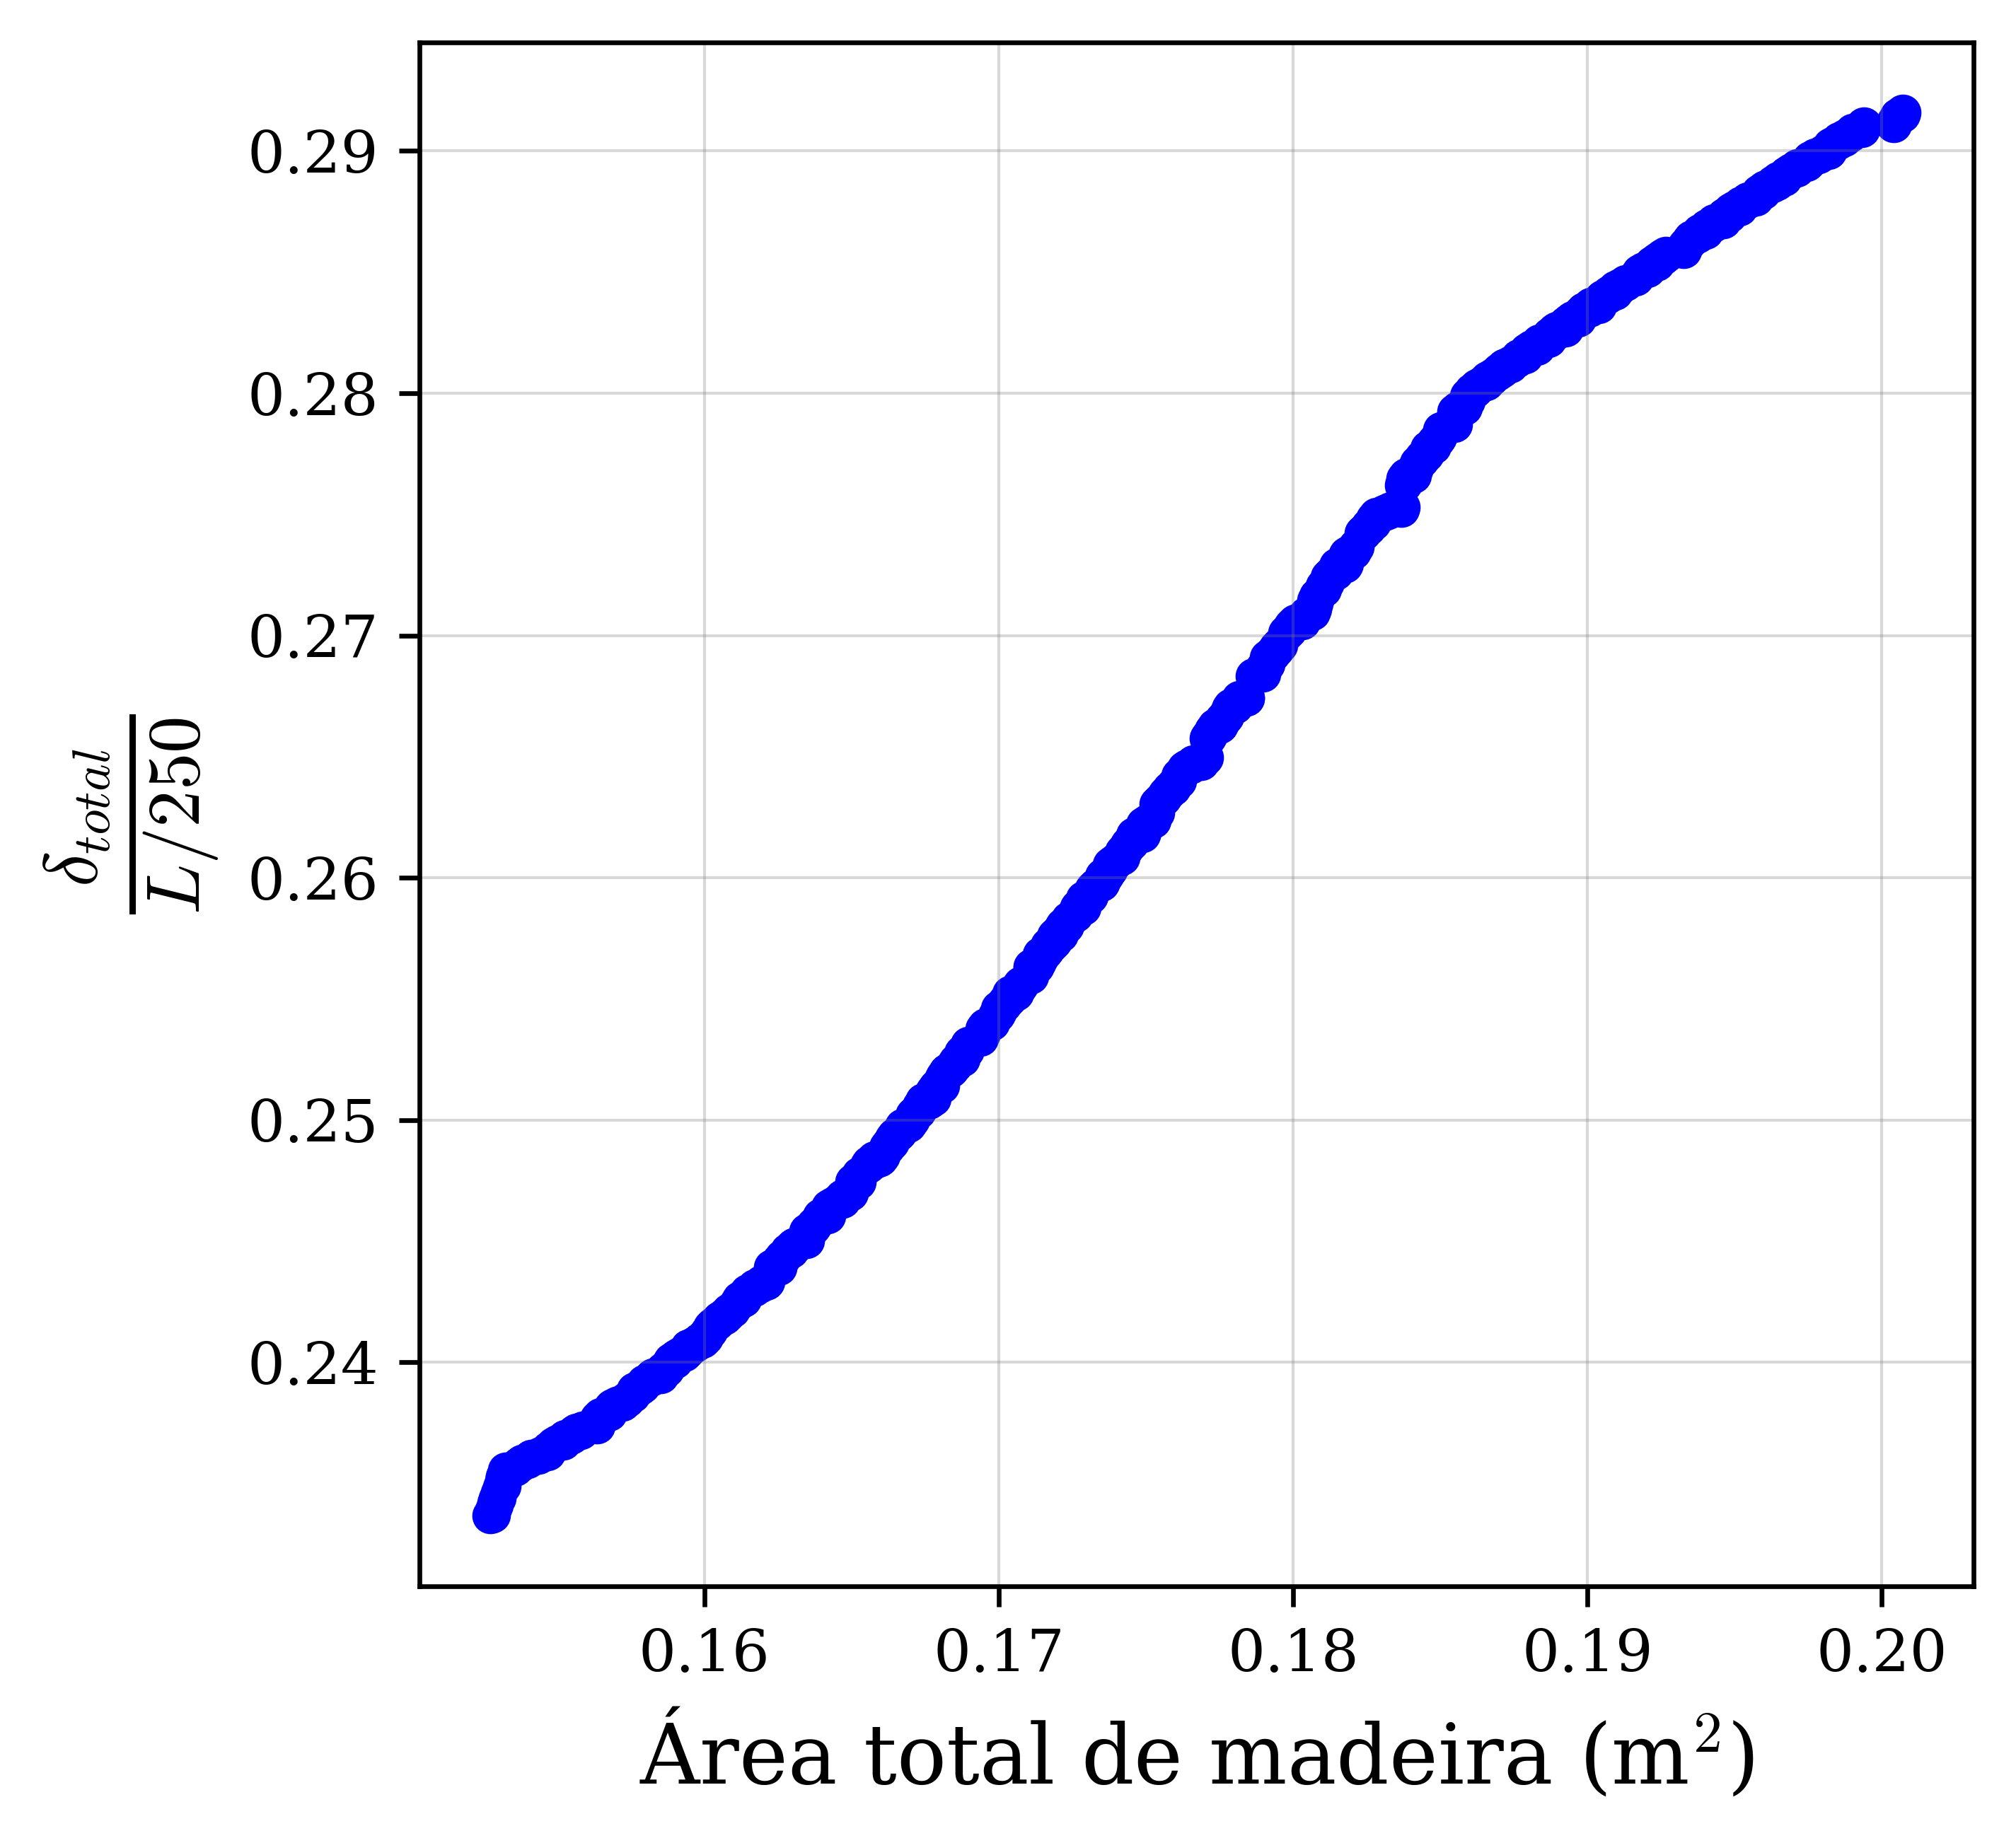
\includegraphics[width=0.55\textwidth]{figuras/z_fronteira_eficiente.png}
    \caption{Fronteira eficiente da Ponte 01 (TB-240).}
    \label{fig:fronteira01}
\end{figure}

Para demonstrar a eficiência do processo de otimização, empregou-se o método de Monte Carlo para gerar um conjunto de soluções obtidas por amostragem aleatória, sem estratégia de otimização. A Figura~\ref{fig:mc01} compara as soluções aleatórias com a fronteira eficiente, evidenciando a superioridade do método otimizado na identificação de soluções dominantes. Enquanto as soluções aleatórias distribuem-se de forma dispersa e majoritariamente dominada, a fronteira de Pareto ocupa a região de menor consumo de material para cada nível de desempenho, explorando de forma racional o limite de serviço.

\begin{figure}[!ht]
    \centering
    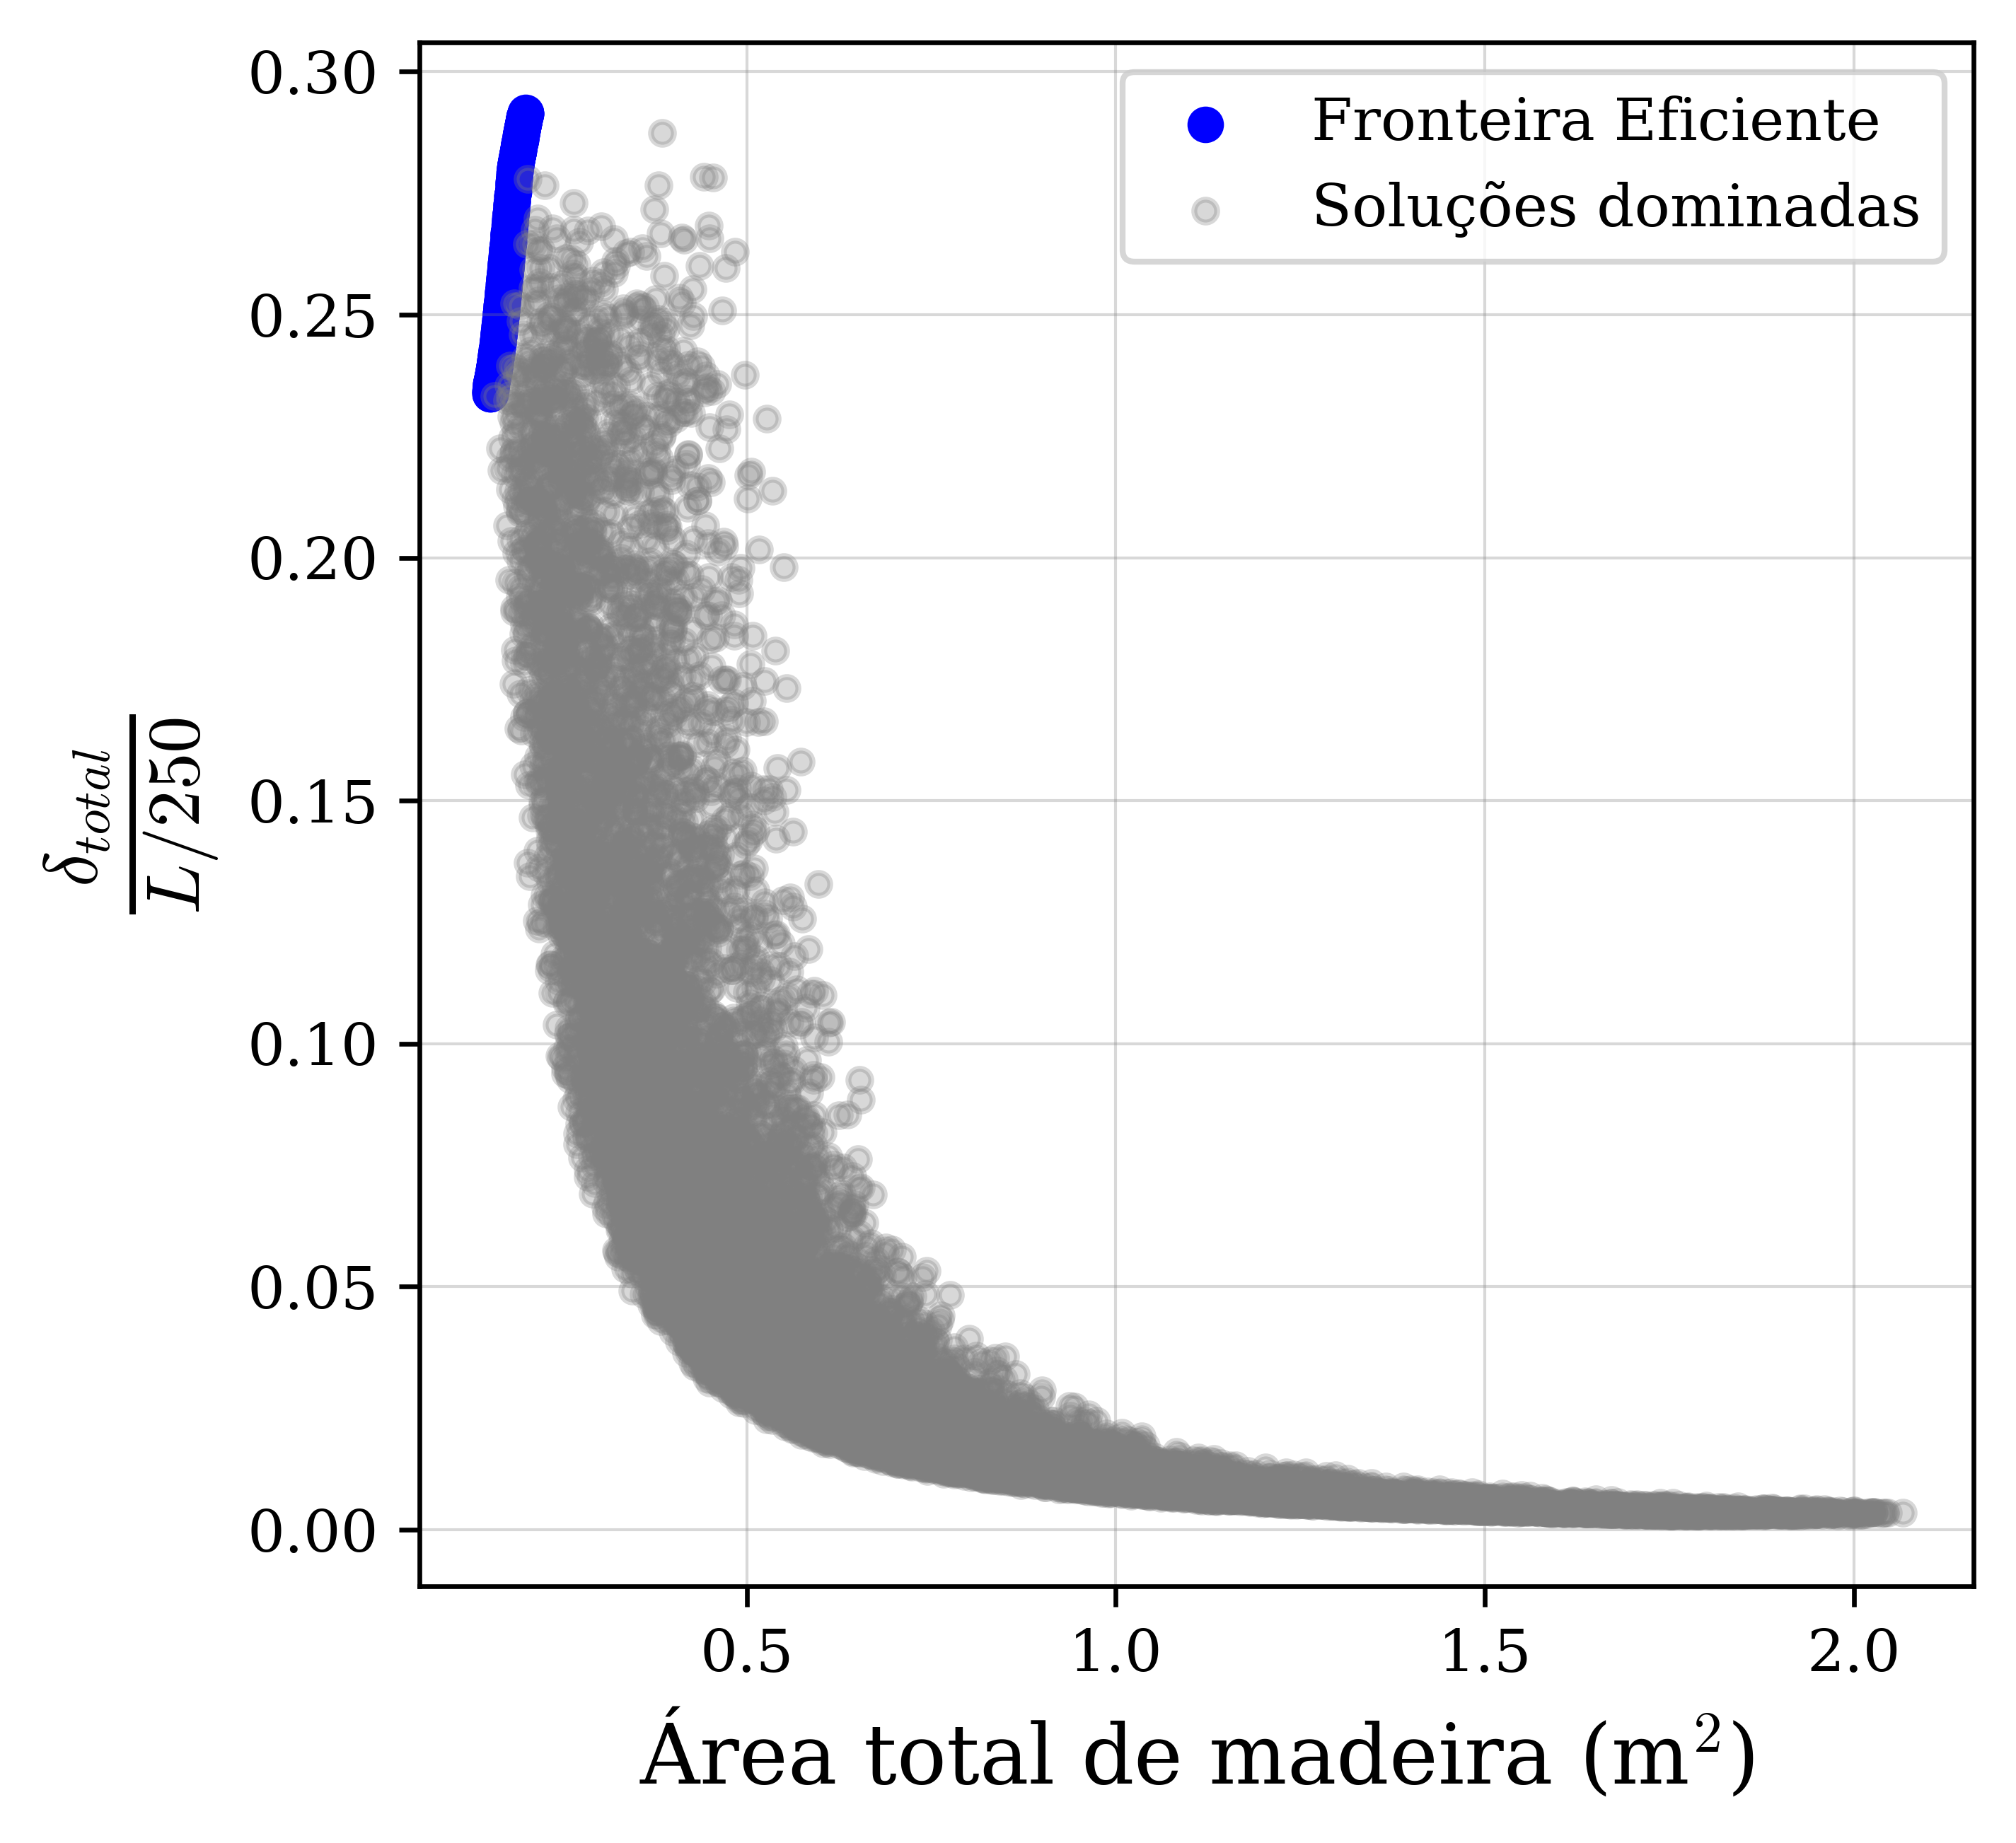
\includegraphics[width=0.55\textwidth]{figuras/z_fronteira_eficiente_vs_monte_carlo.png}
    \caption{Comparação entre a fronteira eficiente e as soluções por Monte Carlo (Ponte 01).}
    \label{fig:mc01}
\end{figure}

\sugestao{Substituir a comparação puramente qualitativa da Figura~\ref{fig:mc01} por métricas quantitativas de qualidade da fronteira: reportar o hipervolume (HV) e o \textit{spacing} da fronteira robusta frente à nuvem de Monte Carlo, e apresentar uma tabela com a redução percentual de área para pelo menos três soluções pareadas (mesmo nível de flecha adimensional). Indicadores de hipervolume são padrão em periódicos de otimização de alto impacto.}

\sugestao{Adicionar gráfico de convergência do NSGA-II para as três configurações de ponte (TB-240, TB-450 e um caso adicional de vão maior), mostrando a evolução do hipervolume em função do número de gerações. Isso demonstra objetivamente a convergência do algoritmo e justifica a escolha de $N_{gen} = 400$.}

\subsection{Fronteira eficiente da Ponte 02 (TB-450)}\label{sec:ponte02}

O processo foi repetido para a Ponte 02, na qual se adota o TB-450 como trem tipo. Os resultados, ilustrados nas Figuras~\ref{fig:fronteira02} e~\ref{fig:mc02}, apresentam comportamento qualitativamente semelhante ao da Ponte 01. A tendência de variação das áreas e das flechas manteve-se consistente, indicando que o modelo computacional responde de maneira coerente à alteração do trem tipo, preservando a relação entre rigidez, consumo de material e deslocamentos máximos.

\begin{figure}[!ht]
    \centering
    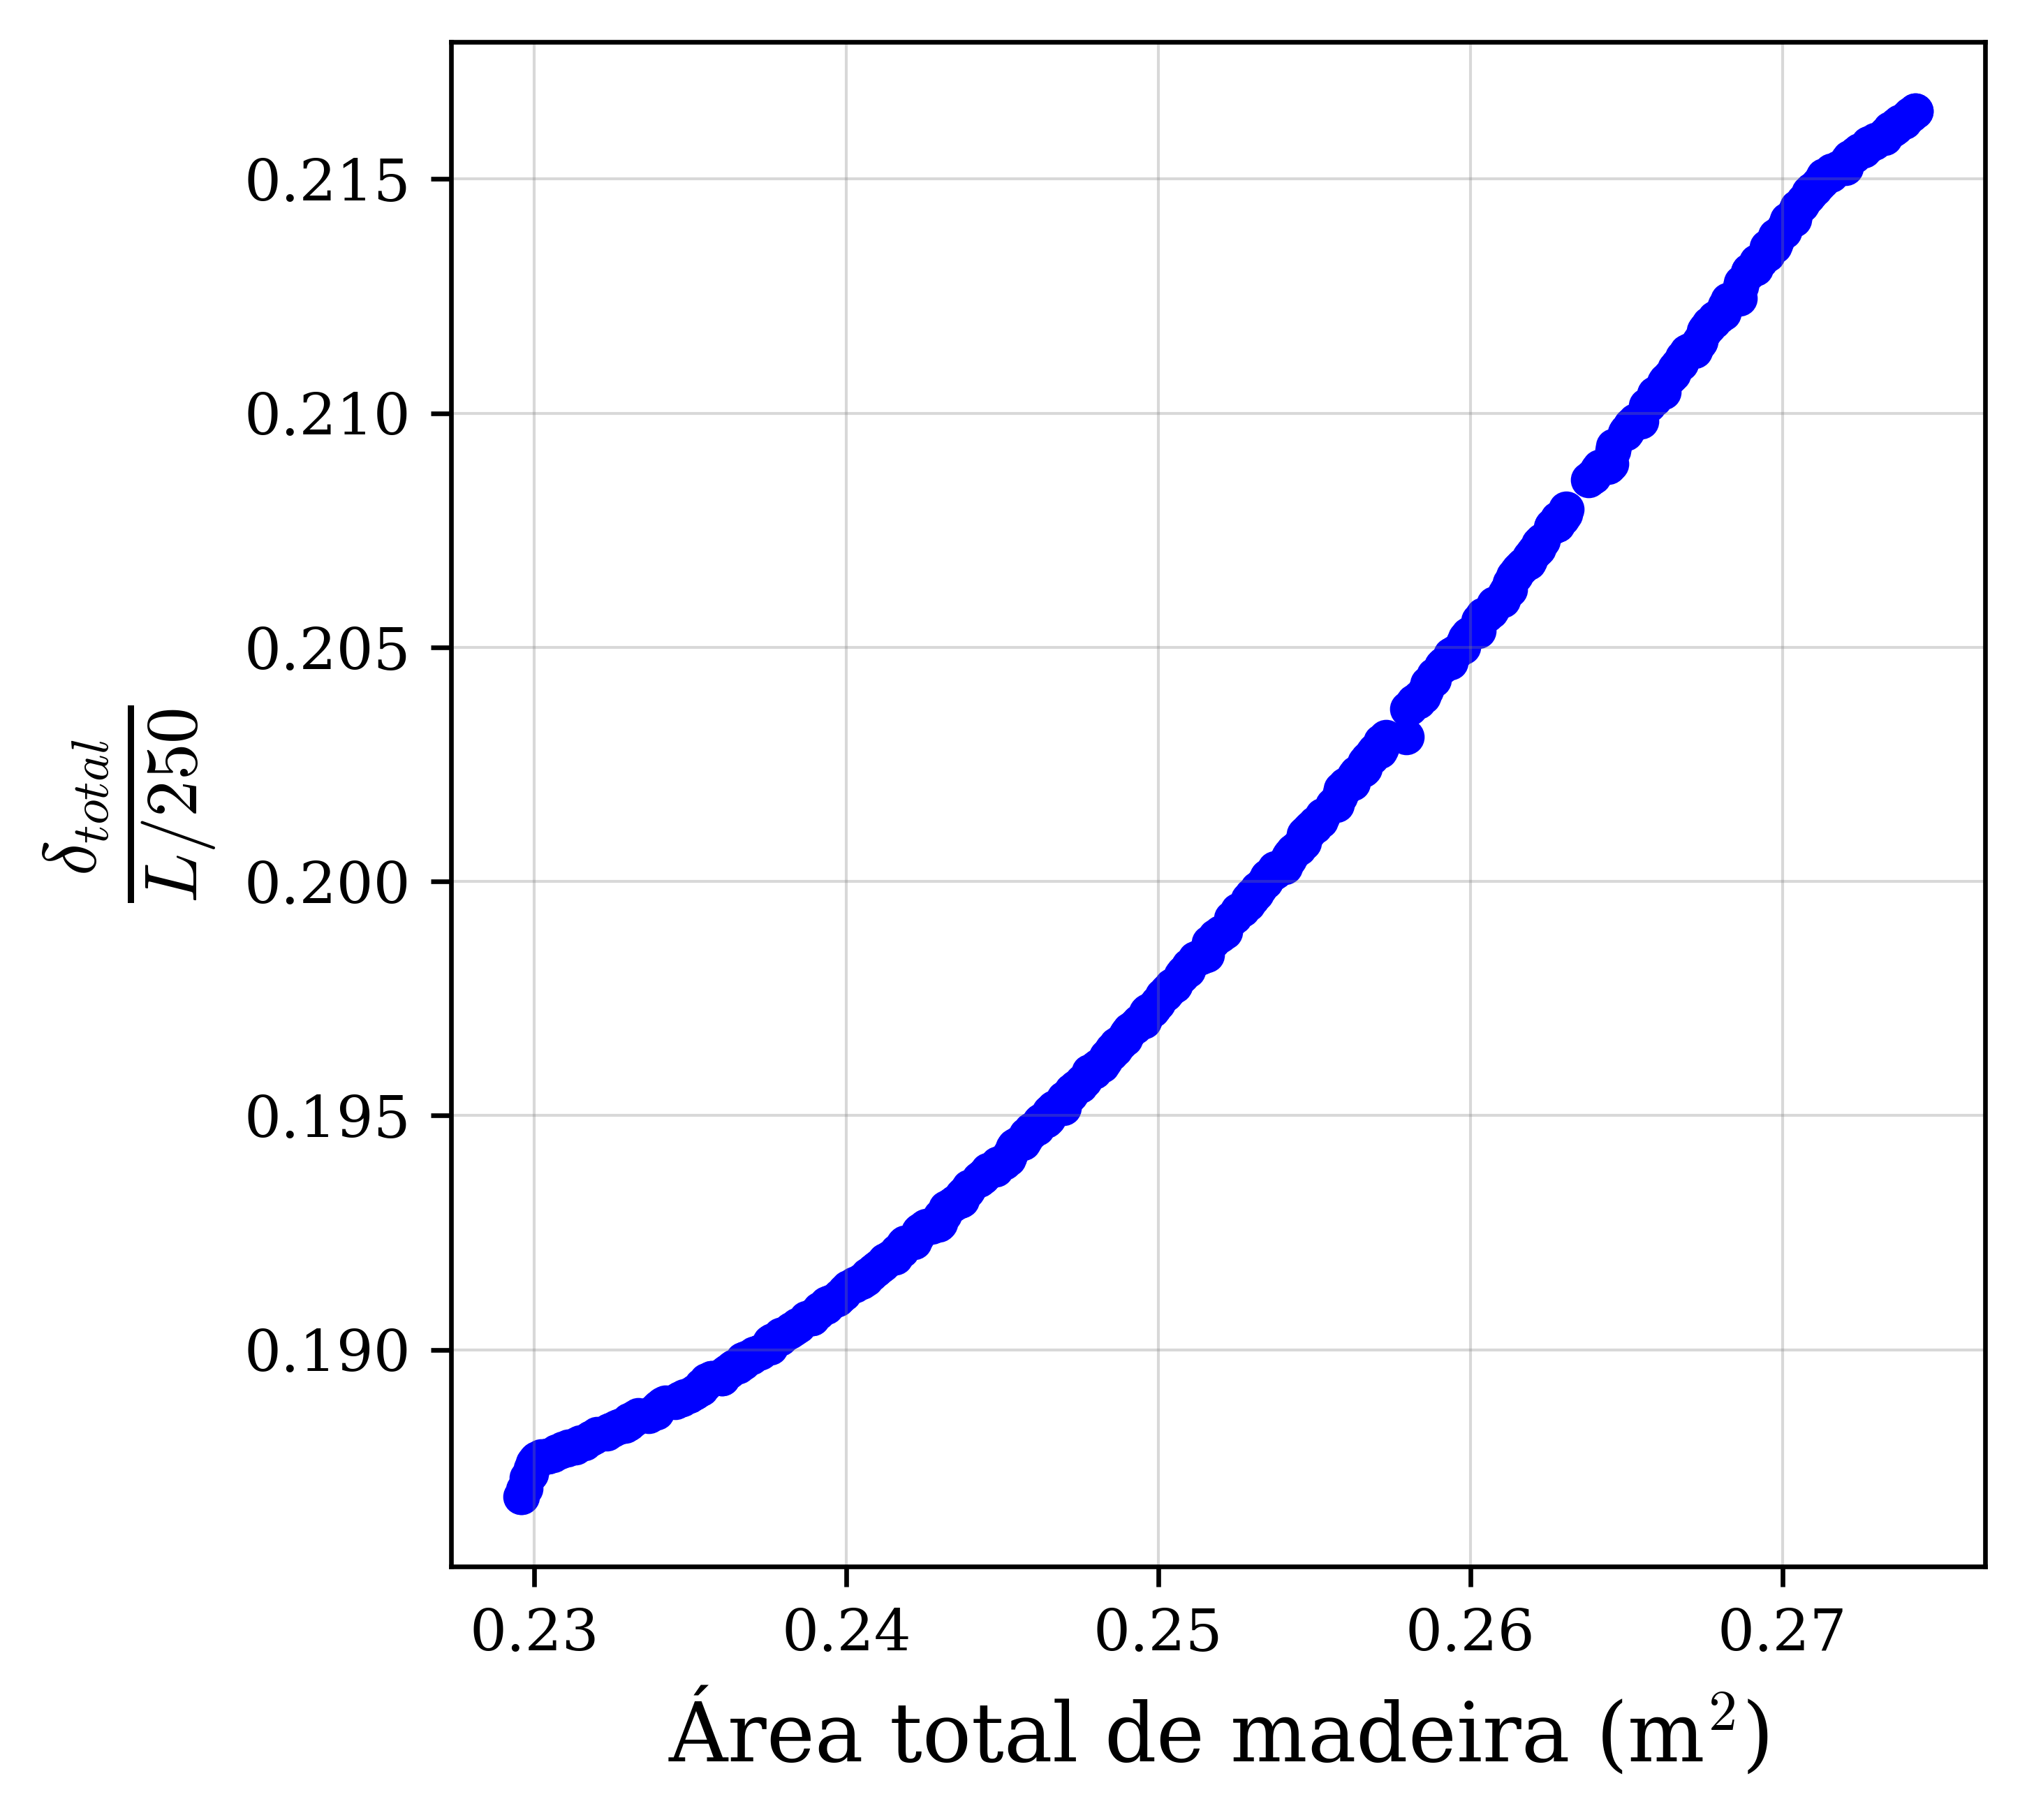
\includegraphics[width=0.55\textwidth]{figuras/z_fronteira_eficiente_viga2.png}
    \caption{Fronteira eficiente da Ponte 02 (TB-450).}
    \label{fig:fronteira02}
\end{figure}

\begin{figure}[!ht]
    \centering
    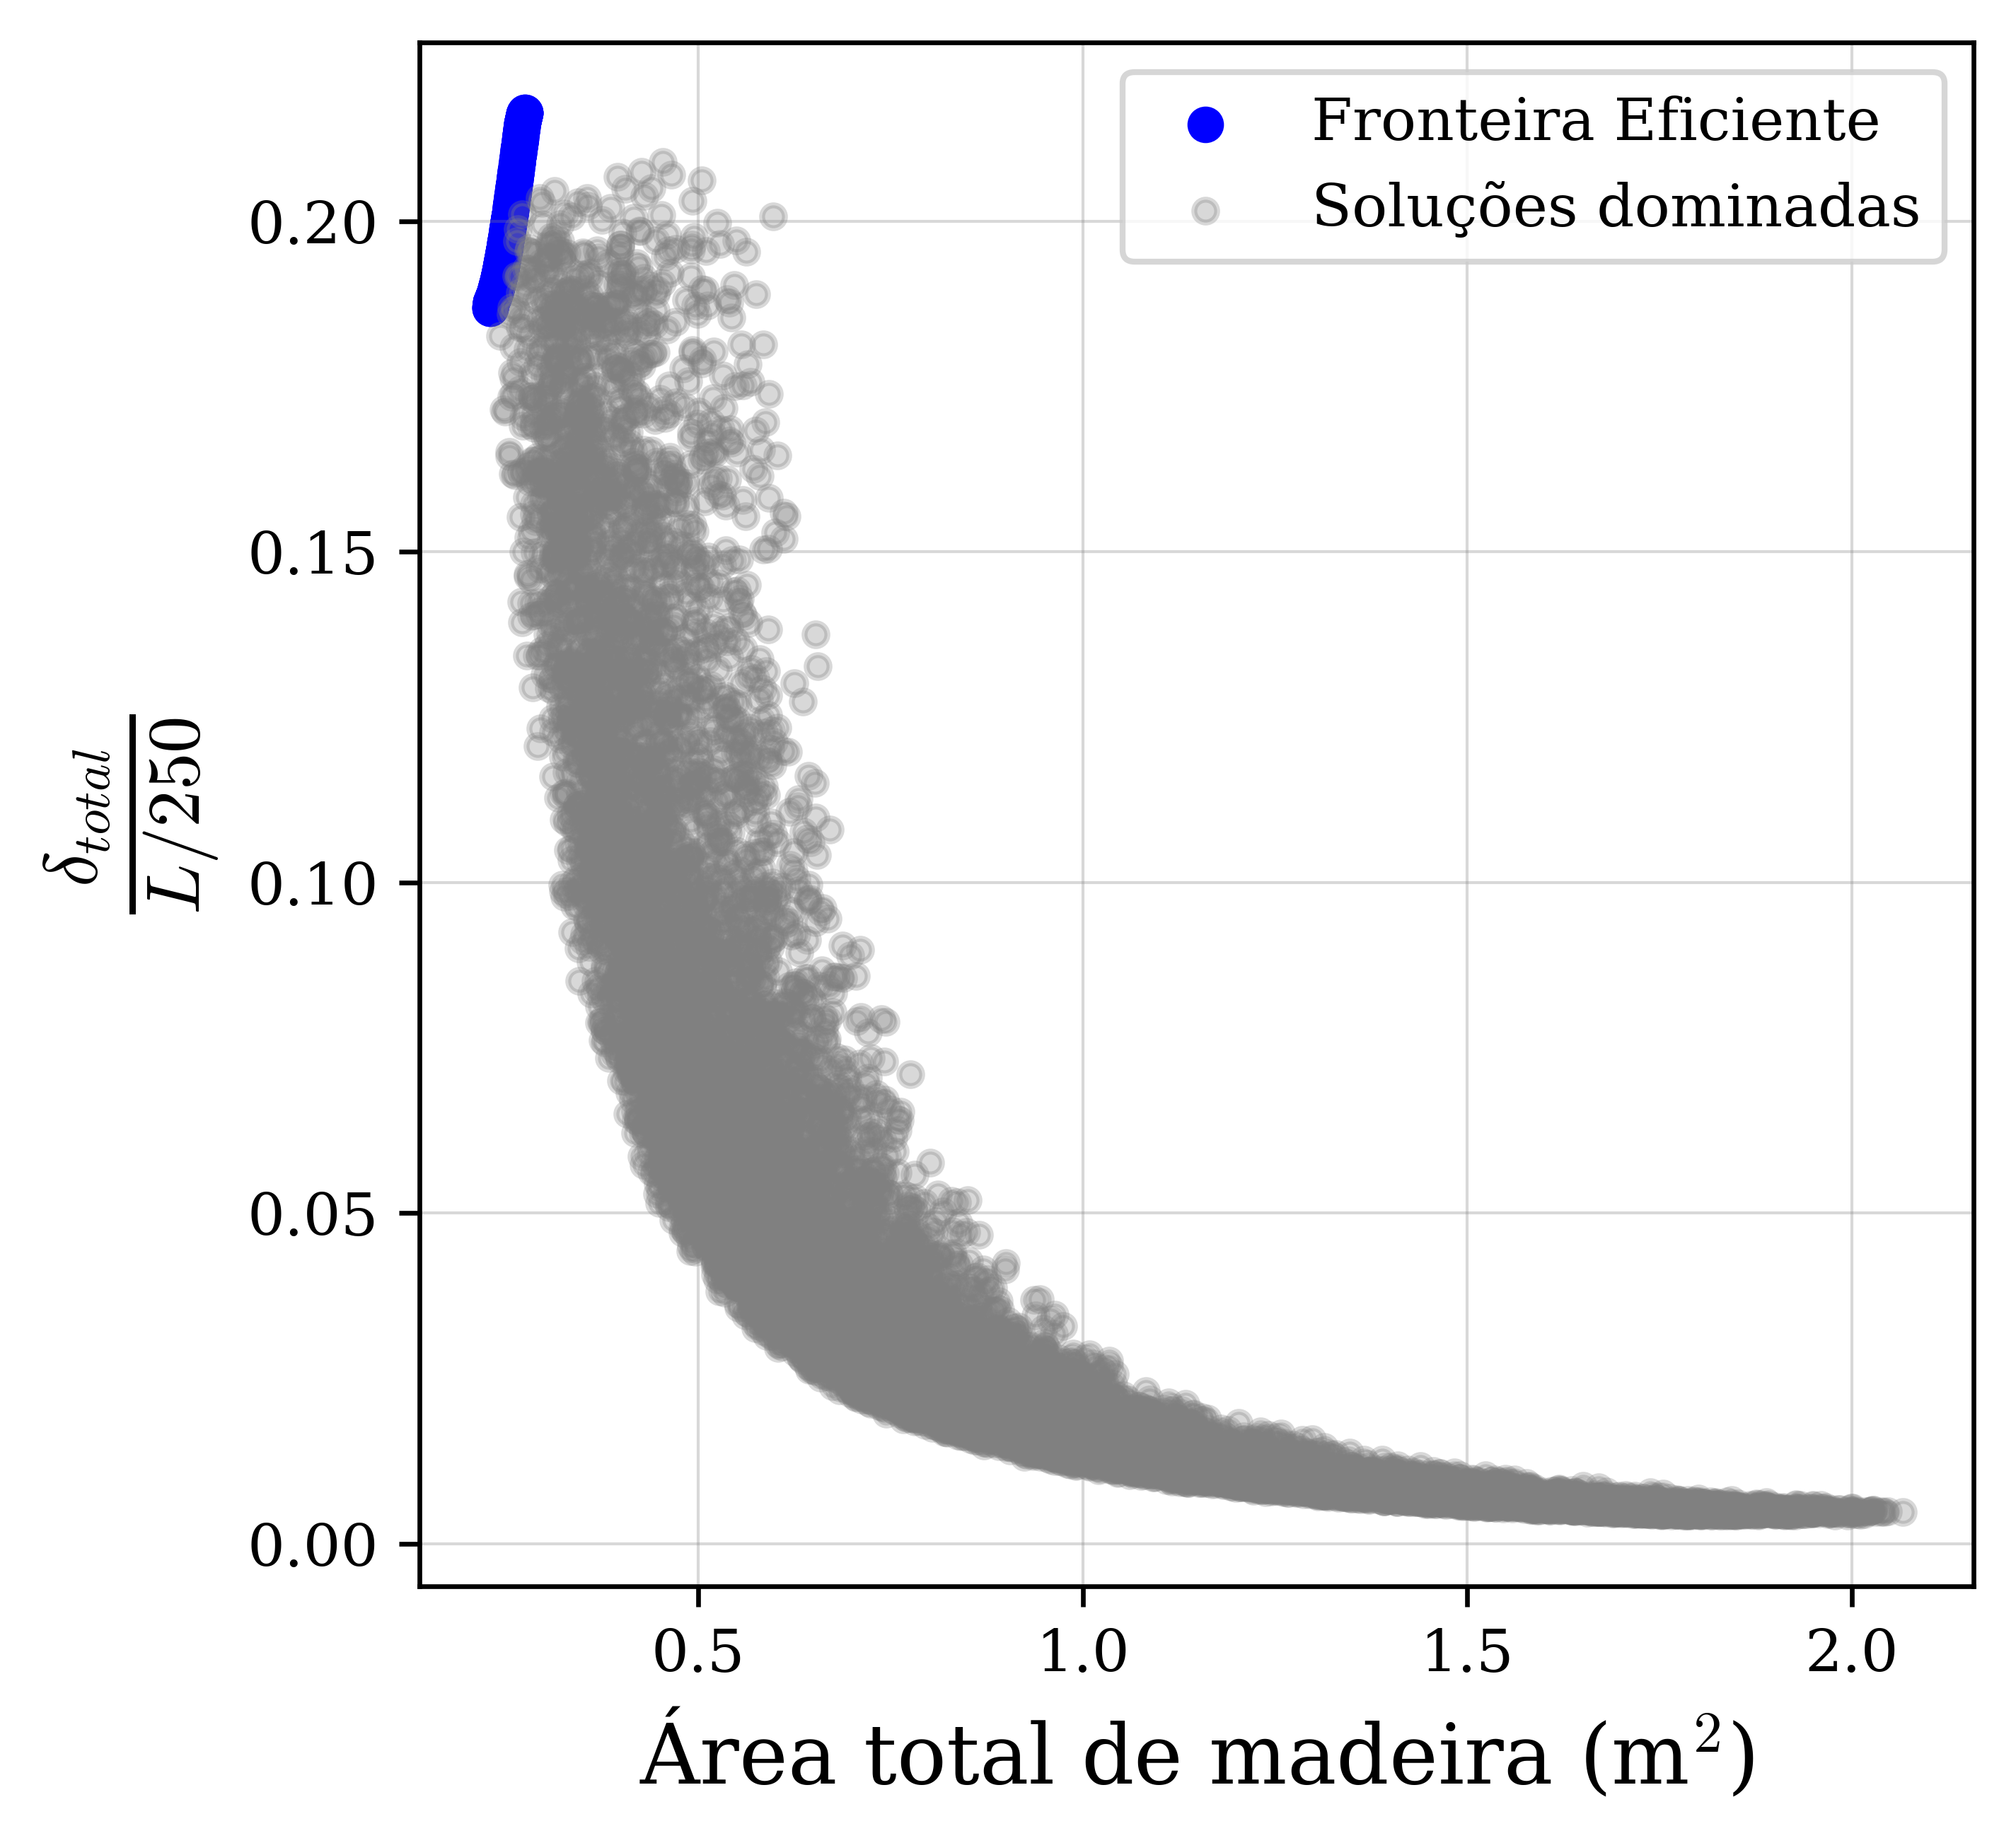
\includegraphics[width=0.55\textwidth]{figuras/z_fronteira_eficiente_vs_monte_carlo_viga2.png}
    \caption{Comparação entre a fronteira eficiente e as soluções por Monte Carlo (Ponte 02).}
    \label{fig:mc02}
\end{figure}

\subsection{Análise comparativa entre os cenários de carregamento}\label{sec:comparacao}

A Tabela~\ref{tab:comparacao} resume as áreas totais de madeira obtidas para cada cenário, incluindo valores mínimos, máximos e médios, bem como os acréscimos percentuais da Ponte 02 em relação à Ponte 01. Ressalta-se que ambas as estruturas possuem a mesma configuração geométrica e propriedades mecânicas, diferenciando-se apenas pelo trem tipo, o que evidencia a influência direta do carregamento móvel nos resultados da otimização.

\begin{table}[!ht]
\caption{Comparação das áreas totais de madeira para os diferentes cenários de carregamento.\label{tab:comparacao}}
\begin{threeparttable}
\begin{tabular*}{\columnwidth}{@{\extracolsep\fill}lccc@{\extracolsep\fill}}
\toprule
Cenário & Mínimo (m\textsuperscript{2}) & Máximo (m\textsuperscript{2}) & Média (m\textsuperscript{2}) \\
\midrule
Ponte 01 (TB-240) & 0{,}16 & 0{,}20 & 0{,}18 \\
Ponte 02 (TB-450) & 0{,}23 & 0{,}27 & 0{,}25 \\
\midrule
Acréscimo (\%) & $+44$ & $+35$ & $+39$ \\
\bottomrule
\end{tabular*}
\end{threeparttable}
\end{table}

A Ponte 01 apresenta áreas totais entre 0{,}16~m\textsuperscript{2} e 0{,}20~m\textsuperscript{2}, enquanto a Ponte 02 apresenta valores entre 0{,}23~m\textsuperscript{2} e 0{,}27~m\textsuperscript{2}. O aumento do carregamento móvel resulta em um acréscimo expressivo no consumo de material ao longo de toda a fronteira eficiente, com incrementos variando entre 35\% e 44\%, e valor médio de aproximadamente 39\%. Esse resultado evidencia o impacto direto do trem tipo mais severo no dimensionamento ótimo das seções. Do ponto de vista do desempenho em serviço, o maior consumo de material na Ponte 02 contribui para a redução relativa do fator de flecha normalizado, indicando maior rigidez global. Em contrapartida, a Ponte 01, ao utilizar seções mais esbeltas, opera mais próxima do limite admissível, caracterizando uma solução mais eficiente em economia de material, porém com menor margem de rigidez.

\subsection{Efeito da otimização robusta}\label{sec:efeito_robustez}

A incorporação da robustez desloca a fronteira eficiente para o interior do domínio viável. Enquanto a otimização determinística tende a produzir soluções com função limite de flexão da longarina exatamente nula ($g_1 \approx 0$), a otimização robusta penaliza essas soluções, pois sob perturbação de $\pm 5\%$ parte das realizações resultaria em violação. Como consequência, as soluções da fronteira robusta apresentam pequena folga adicional nas restrições ativas, garantindo que permaneçam seguras mesmo diante da variabilidade dimensional da madeira roliça, ao custo de um acréscimo controlado no consumo de material.

\sugestao{Apresentar figura sobrepondo a fronteira determinística ($\rho = 0\%$) e a fronteira robusta ($\rho = 5\%$) para a Ponte 01, com uma tabela quantificando o acréscimo médio de área (custo da robustez) e a redução da probabilidade de falha $p_f$ de soluções selecionadas. Este é o resultado central de originalidade do trabalho e deve receber destaque para atingir periódicos de alto impacto (JCR elevado).}

\sugestao{Realizar uma validação por simulação de Monte Carlo independente: para uma solução da fronteira determinística e uma da fronteira robusta com mesma área, aplicar 10\textsuperscript{4} perturbações de $\pm 5\%$ e reportar o percentual de realizações que violam cada restrição, demonstrando empiricamente o ganho de robustez.}

\sugestao{Incluir análise de sensibilidade global (índices de Sobol) das variáveis de projeto sobre as funções limite, identificando quais variáveis mais contribuem para a violação das restrições sob perturbação, o que orienta o controle de qualidade na fabricação das peças de madeira roliça.}

\sugestao{Estender a comparação a um estudo de caso com ponte real de estrada vicinal, confrontando o consumo de material da solução otimizada robusta com o projeto executado, à semelhança das validações em pontes existentes reportadas na literatura de projeto paramétrico de pontes.}
